\section{Microcontroller Basics}

\subsection{Microcontroller Architecture}

\mult{2}

\begin{theorem}{Embedded Systems}
    \begin{itemize}
        \item low cost (usb sticks, consumer electronics)
        \item low power (sensor networks, mobile devices)
        \item small size (smart cards, wearables)
        \item real time (anti-lock brakes, process control)
        \item reliability (medical devices, automotive)
        \item extreme environment (space, automotive)
    \end{itemize}
\end{theorem}

\begin{concept}{Single Chip Solution} \\
    $\Rightarrow$ CPU with integrated memory and peripherals
\end{concept}

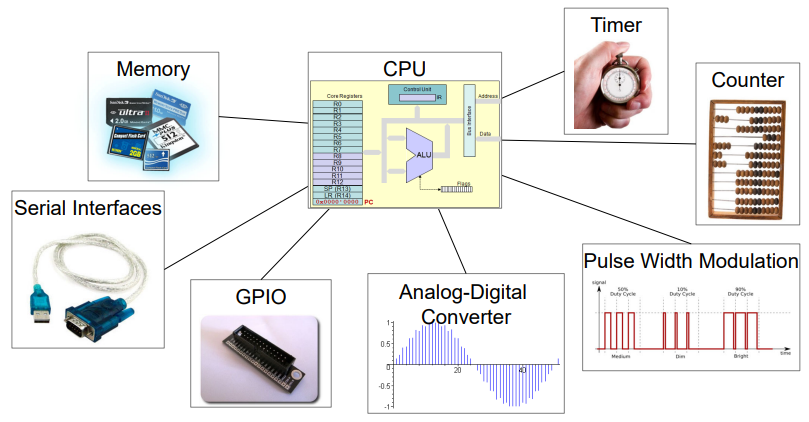
\includegraphics[width=\linewidth]{single_chip_solution.png}

\multend

\subsubsection{Peripherals and Registers}

\begin{definition}{Peripherals}

    \begin{minipage}{0.35\linewidth}
    \begin{itemize}
        \item configurable hardware blocks \\ of a microcontroller
        \item accepts specific task from CPU, \\ executes task and returns result \\ (status, e.g. task completion, error)
        \item often interfaces to outside world\\
        many (not all) interact with \\ external MCU pins 
        \item examples: GPIO, UART, SPI, ADC
    \end{itemize}
    \end{minipage}
    \begin{minipage}{0.64\linewidth}
        \vspace{-5mm}
        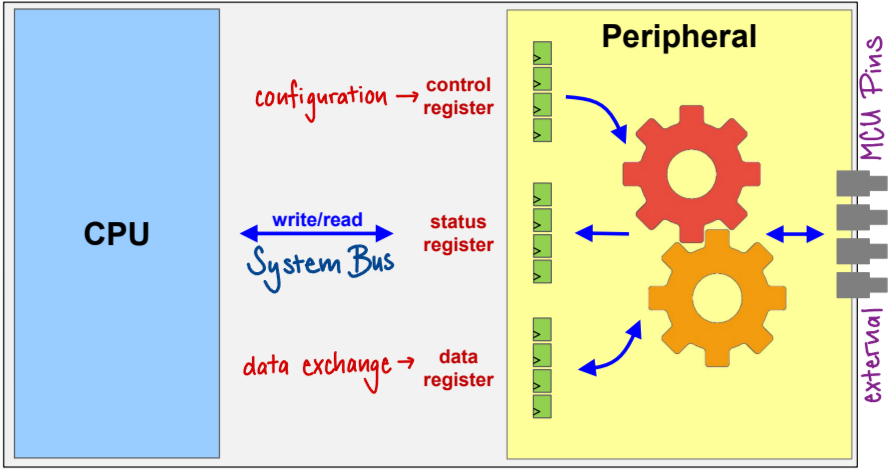
\includegraphics[width=\linewidth]{peripherals_registers.png}
    \end{minipage}
\end{definition}

\mult{2}

\begin{definition}{Registers}
    \begin{itemize}
        \item Registers are arrays of flip-flops (storage elements with two states, i.e. 0 or 1)
        \item Each flip-flop stores one bit of information
        \item CPU writes to and reads from registers
    \end{itemize}
\end{definition}

\begin{theorem}{CPU read/write to peripheral registers}\\
    How does the CPU write to and read from peripheral registers?
    \vspace{-2mm}\\
    \begin{itemize}
        \item CPU reads/writes to peripheral registers
        \item CPU uses memory-mapped I/O to access peripheral registers
        \item CPU uses load/store instructions to access peripheral registers
    \end{itemize}
    $\Rightarrow$ System Buses
\end{theorem}

\begin{concept}{Control and Status Registers}\\
Peripherals interact with the CPU through registers:
\begin{itemize}
    \item \textbf{Control Registers}: CPU configures peripherals
    \begin{itemize}
        \item CPU writes to register bit
        \item Slave hardware uses the output of this bit
        \item Usually read/write
    \end{itemize}
    \item \textbf{Status Registers}: CPU monitors peripheral state
    \begin{itemize}
        \item Slave writes status into register bit
        \item CPU reads register bit
        \item Usually read-only
    \end{itemize}
\end{itemize}
Both control \& status bits can be in same register.
\begin{itemize}
    \item \textbf{Data Registers} \\
        enable CPU to exchange data with the peripheral
\end{itemize}
\end{concept}

\raggedcolumns
\multend

\begin{concept}{CPU access to individual Peripheral Registers}
    \begin{itemize}
        \item ARM \& STM map the peripheral registers into
        the memory address range
        \item Reference Manual shows the defined addresses
    \end{itemize}
    \vspace{2mm}
    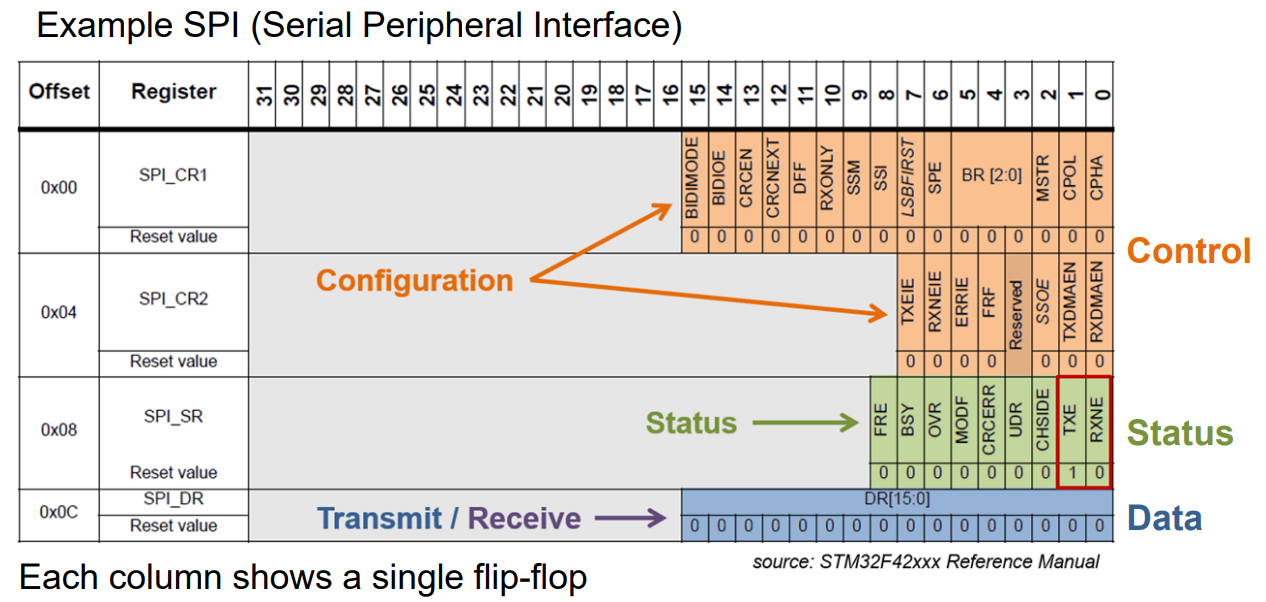
\includegraphics[width=\linewidth]{example_SPI_cpu_access.png}
\end{concept}

\mult{2}

\begin{definition}{Memory mapping of Peripheral Registers}
    \begin{itemize}
        \item Each peripheral register has a unique address
        \item CPU uses the address to access the register
        \item CPU uses load/store instructions to access the register
    \end{itemize}
    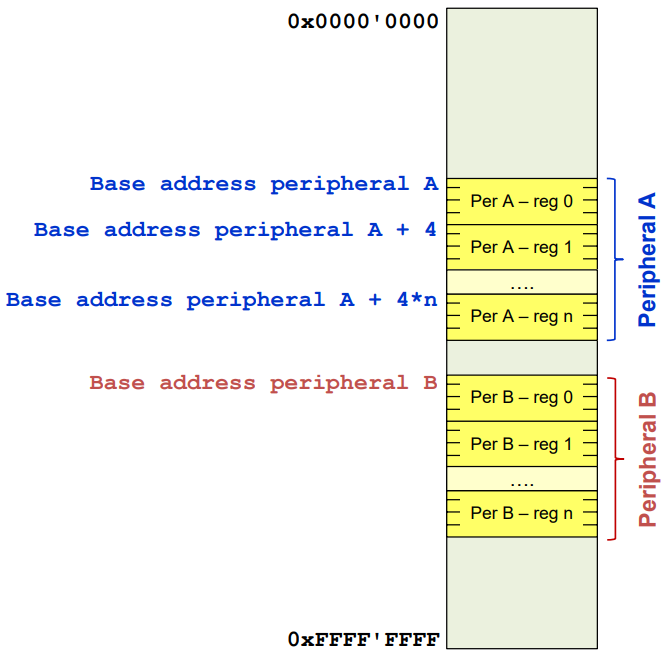
\includegraphics[width=\linewidth]{peripheral_registers_cpu_access.png}
\end{definition}

\begin{definition}{Memory-Mapped Peripheral Registers}
    \begin{itemize}
        \item Control register: controls states of LEDs
        \item Status register: monitors states of DIP switches
    \end{itemize}
    \vspace{1mm}
    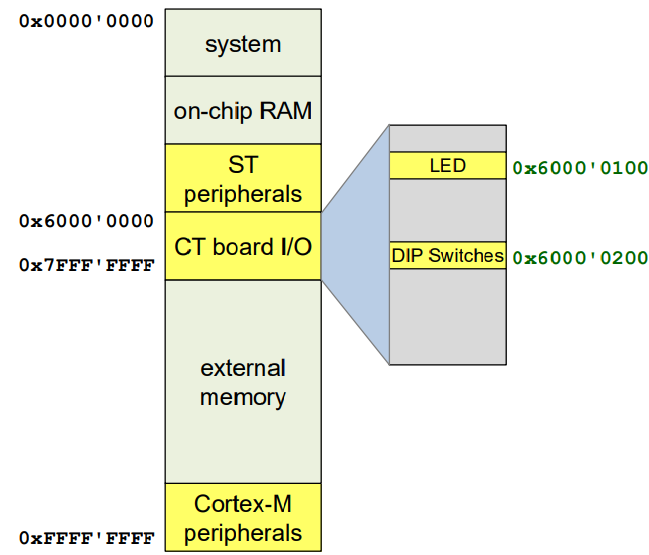
\includegraphics[width=\linewidth]{registers_leds_dipswitches.png}
\end{definition}

\multend

\begin{code}{Memory-Mapped Registers}\\
Registers are mapped into the memory address range - each has a specific address:
\begin{lstlisting}[language=C, style=basesmol]
// Define memory-mapped register addresses
#define ADDR_LED_31_0       0x60000100
#define ADDR_DIP_SWITCH_31_0 0x60000200

// Read from DIP switches and write to LEDs
uint32_t value = read_word(ADDR_DIP_SWITCH_31_0);
write_word(ADDR_LED_31_0, value);
\end{lstlisting}
\end{code}


\subsubsection{System Bus}
\mult{2}


\begin{definition}{System Bus}
    \begin{itemize}
        \item Interconnects CPU with memory and peripherals, \\allowing data transfer between components.
        \item CPU acts as master: initiating and controlling all transfers
        \item Peripherals and memory act as slaves: responding to requests from the CPU
        \item System bus is a shared resource
    \end{itemize}
    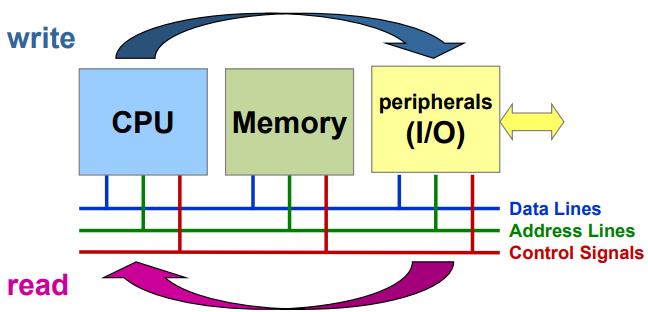
\includegraphics[width=\linewidth]{system_bus.png}\\
    The CPU acts as a master, initiating and controlling all transfers, while peripherals and memory act as slaves, responding to requests.
\end{definition}



\begin{theorem}{Signal Groups}
    \begin{itemize}
        \item \textcolor{darkblue}{\textbf{Data lines}}
        \begin{itemize}
            \item Bidirectional (read/write)
            \item Number of lines $\rightarrow$ data bus width \\(8, 16, 32, 64 parallel lines of data)
            \item Example: Cortex-M has 32 address lines $\rightarrow$ 4GB address space \\ $\rightarrow$ \texttt{0x00000000} to \texttt{0xFFFFFFFF}
        \end{itemize}
        \item \textcolor{darkgreen}{\textbf{Address lines}}
        \begin{itemize}
            \item Unidirectional: from Master to slaves
            \item Number of lines $\rightarrow$ size of address space \\ (e.g., 32 lines allow $2^{32}$ addresses)
        \end{itemize}
        \item \textcolor{darkred}{\textbf{Control signals}}
        \begin{itemize}
            \item Control read/write direction
            \item Provide timing information
            \item Chip select, read/write, etc.
        \end{itemize}
    \end{itemize}
    \vspace{2mm}
    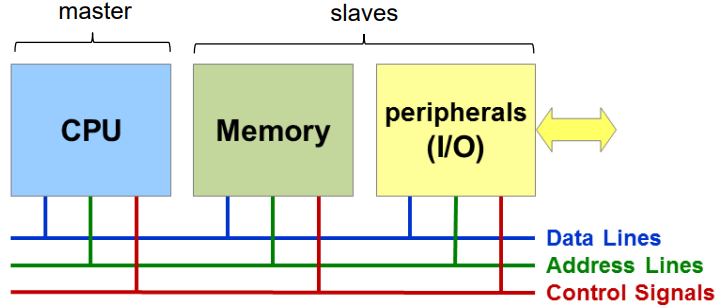
\includegraphics[width=\linewidth]{master_slave_signal_groups.png}
\end{theorem}

\begin{concept}{Bus Specification}
    \begin{itemize}
        \item \textcolor{darkblue}{\textbf{Protocol and operations}}
        \item \textcolor{darkred}{\textbf{Signals}}
        \begin{itemize}
            \item Number of Signals
            \item Signal descriptions
        \end{itemize}
        \item \textcolor{darkgreen}{\textbf{Timing}}
        \begin{itemize}
            \item Frequency
            \item Setup and hold times
        \end{itemize}
        \item \textcolor{darkpurple}{\textbf{Electrical properties}} (not in exam)
        \begin{itemize}
            \item Drive strength and Load
        \end{itemize}
        \item \textcolor{darkorange}{\textbf{Mechanical requirements}} (not in exam)
    \end{itemize}
\end{concept}

\columnbreak

\begin{theorem}{Bus Timing Options}\\
    \textbf{Synchronous}
    \begin{itemize}
        \item \textcolor{blue}{Master} and \textcolor{darkcorn}{slaves} use a common clock\\
        Often dedicated CLK signal from master to slave, \\ but clock can also be encoded in a data signal
        \item Clock edges control bus transfer on both sides
        \item Used by most on-chip buses
        \item Off-chip: DDR and synchronous RAM
    \end{itemize}
    \begin{center}
    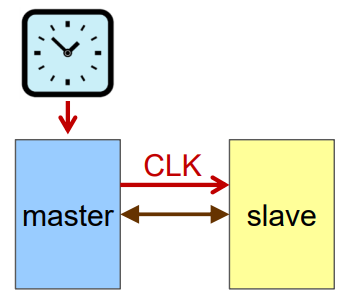
\includegraphics[width=0.6\linewidth]{synchronous_bus_timing.png}
    \end{center}
    \textbf{Asynchronous}
    \begin{itemize}
        \item \textcolor{darkcorn}{Slaves} have no access to clock of the \textcolor{blue}{master}
        \\ $\rightarrow$ slave has their own clock or no clock at all
        \item Control signals carry timing information to allow synchronization
        \item Widely used for low data-rate off-chip memories \\
        $\rightarrow$ parallel flash memories and asynchronous RAM
    \end{itemize}
    \begin{center}
        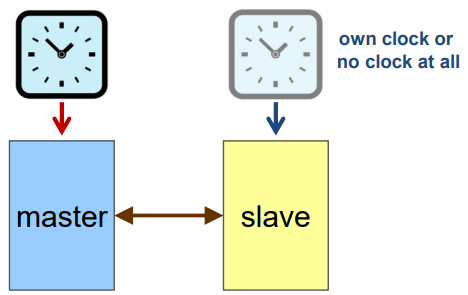
\includegraphics[width=0.6\linewidth]{asynchronous_bus_timing.png}
    \end{center}
\end{theorem}

\important{But how can a driver be disconnected electrically?}

\begin{corollary}{Multiple devices driving the same data line}\\
    What if one device drives a logic 1 (Vcc) and another device drives a logic 0 (Gnd)?\\
    $\Rightarrow$ Electrical short circuit!
    \\ $\rightarrow$ bus contention ('Streitigkeit')\\
    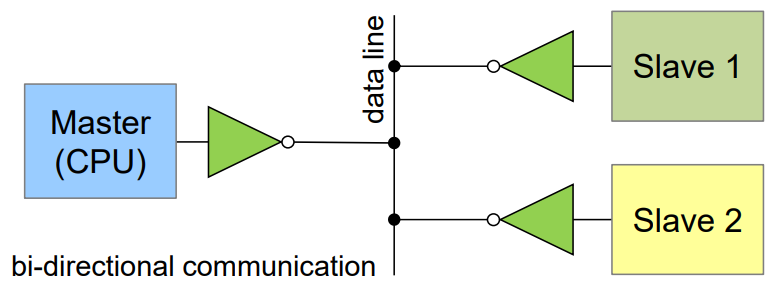
\includegraphics[width=\linewidth]{bus_contention.png}\\
    \small{Figure only shows output paths, input paths are not shown.}

\end{corollary}



\multend


\subsection{Digital Logic Basics}

\mult{2}

\begin{definition}{CMOS Inverter}
    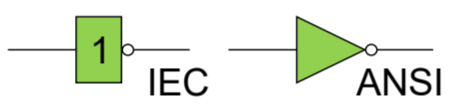
\includegraphics[width=0.5\linewidth]{cmos_inverter0.png}\\
    Complementary switches (transistors)\\
    $\rightarrow$ \textcolor{red}{p-type} and \textcolor{blue}{n-type} have opposite open-close behaviour\\
    \\
    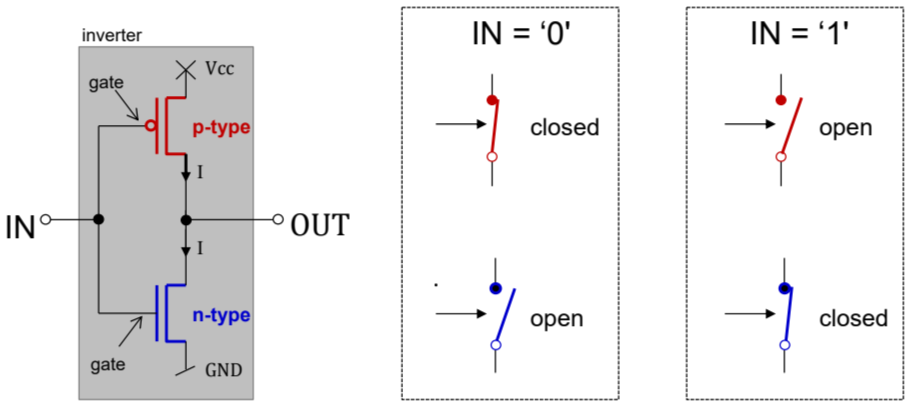
\includegraphics[width=\linewidth]{cmos_inverter1.png}\\
    e.g. Vcc = 3V = '1', Gnd = 0V = '0'\\
    Vcc is the supply voltage of the circuit/chip
    \vspace{2mm}\\
    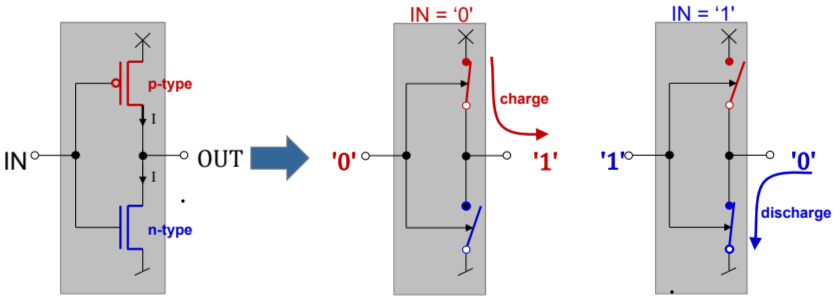
\includegraphics[width=\linewidth]{cmos_inverter2.png}\\
    A buffer is built by connecting two inverters in series
\end{definition}

\begin{definition}{CMOS Tri-State Inverter}\\
    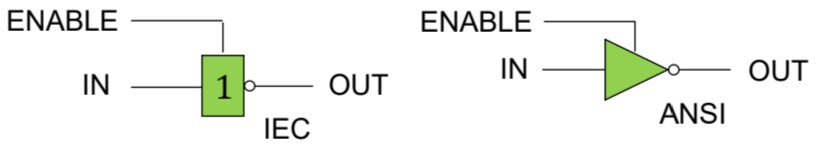
\includegraphics[width=\linewidth]{tristate_inverter1.png}\\
    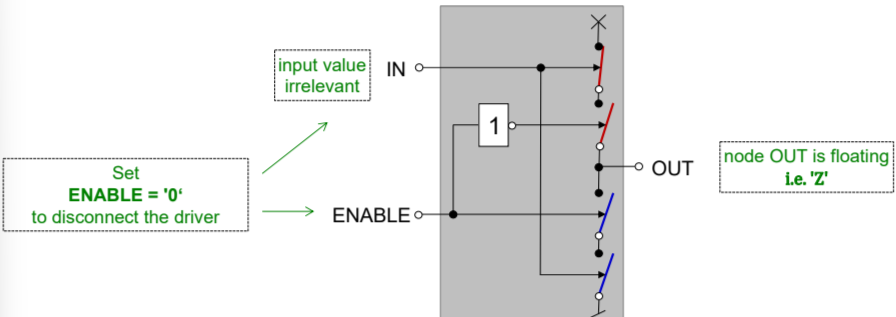
\includegraphics[width=\linewidth]{tristate_inverter3.png}\\
    Implementation:\\
    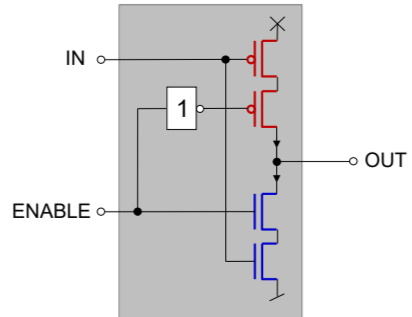
\includegraphics[width=\linewidth]{tristate_inverter4.png}
\end{definition}

\begin{definition}{Tri-State Logic}\\
Multiple devices can drive the same data line thanks to tri-state capability:
\begin{itemize}
    \item Logic '1': Voltage level (e.g., 3.3V)
    \item Logic '0': Ground (0V)
    \item Third state 'Z': High impedance (disconnected, floating)
\end{itemize}
The CPU defines which device drives the bus:
\begin{itemize}
    \item \textbf{Write}: CPU drives bus, all slave drivers disconnected
    \item \textbf{Read}: CPU driver disconnected, selected slave drives bus, other slave drivers disconnected
\end{itemize}
\end{definition}


\begin{concept}{Tri-State Buffer} Timing Diagram\\
    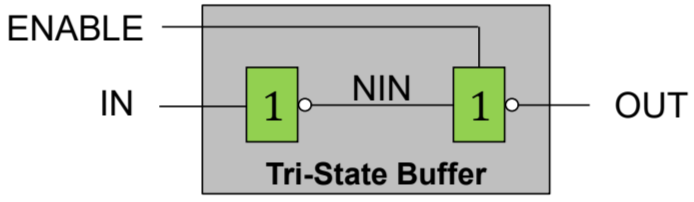
\includegraphics[width=\linewidth]{tristate_buffer1.png}\\
    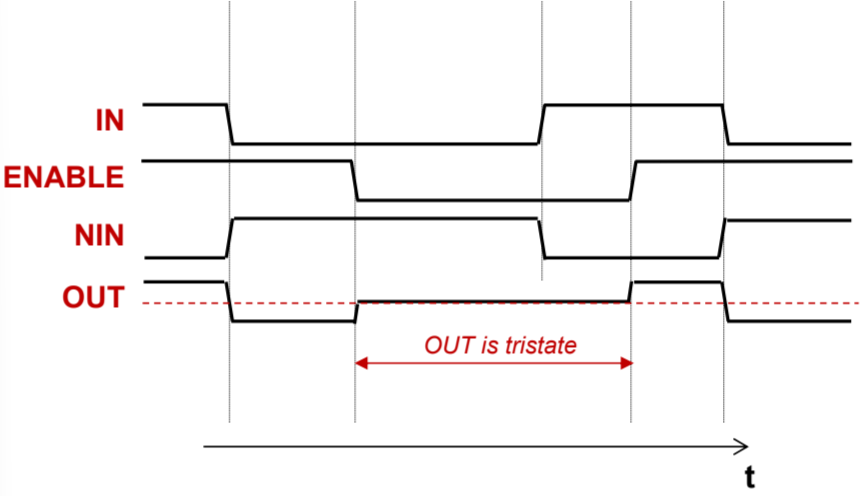
\includegraphics[width=\linewidth]{tristatebuffer2.png}\\
    When a signal like OUT is in tristate, we often say that it is 'floating'. 
    The term expresses that such a signal can easily be moved by parasitic electrical effects
    to either one of the reference levels, i.e. '0' or '1'.
\end{concept}

\begin{KR}{Bus Contention} \\
    CPU defines who drives the data bus at which moment in time:
    \begin{itemize}
        \item \texttt{write} CPU drives bus $\rightarrow$ all slave drivers disconnected
        \item \texttt{read} CPU releases bus $\rightarrow$ one slave drives bus (selected through values on address lines, other slave drivers disconnected)
    \end{itemize}
    
    Electrically disconnecting a driver is called \textbf{tri-state} or \textbf{high-impedance} (Hi-Z) state. (switch)
    
    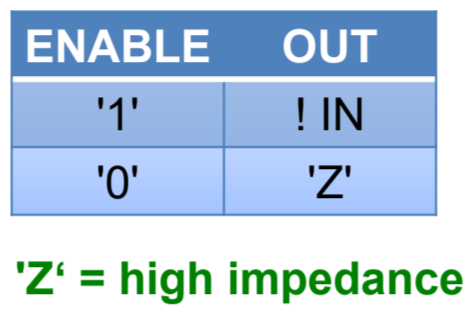
\includegraphics[width=0.5\linewidth]{tristate_inverter2.png}\\
\end{KR}



\multend

\subsection{Synchronous Bus}

\mult{2}

\begin{definition}{Synchronous Bus}\\
    Example Uses External Bus from ST Microelectronics
    \begin{itemize}
        \item Reason: Internal workings of the system bus are not disclosed by STM
        \item Signal names, bus protocol and timing based on external synchronous STM32F429xx mode instead
        \item For details see Chapter 37, Flexible memory controller (FMC) in ST Reference Manual RM0090
        \item Datasheet STM32F429xx
        \item Figure 60 Synchronous non-multiplexed NOR/PSRAM read timings
        \item Figure 61 Synchronous non-multiplexed PSRAM write timings
    \end{itemize}
Naming Convention
\begin{itemize}
    \item Letter ' N ' prefix in signal name ( $\mathrm{N} x x x$ ) means active-low signal
    \item E.g. NOE means 'NOT OUTPUT ENABLE'
\end{itemize}

NOE $=$ ' 0 ' $\rightarrow$ output enabled\\
NOE $=$ ' 1 ' $\rightarrow$ output disabled
\end{definition}

\begin{concept}{Synchronous Bus Timing}\\
Key signals for read/write operation:
\begin{itemize}
    \item \textbf{CLK}: System clock
    \item \textbf{A[31:0]}: Address lines
    \item \textbf{D[31:0]}: Data lines
    \item \textbf{NWE}: Not Write Enable (active low)
    \item \textbf{NOE}: Not Output Enable (active low)
    \item \textbf{NE}: Not Enable (active low)
\end{itemize}
Note that 'N' prefix indicates active-low signals.
\end{concept}



\begin{formula}{Block Diagram}\\
    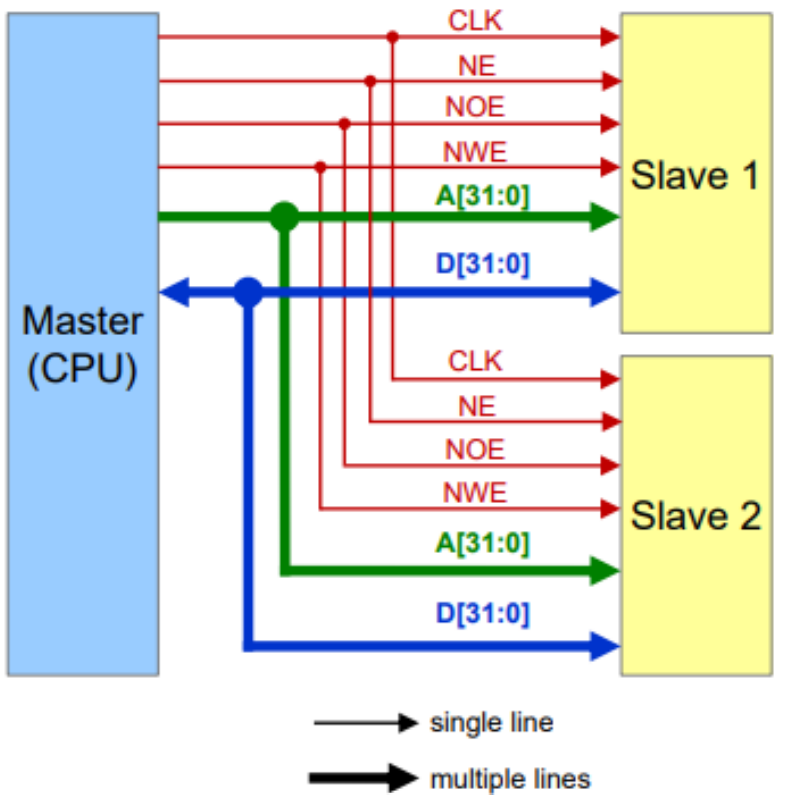
\includegraphics[width=\linewidth]{block_diagramm.png}
\end{formula}

\begin{definition}{Bus Timing Diagram}
    \begin{itemize}
        \item CLK $\rightarrow$ clock signal (rising edge)
        \item NE $\rightarrow$ Not enable (active low)
        \item NWE $\rightarrow$ Not write enable (active low)
        \item NOE $\rightarrow$ Not output enable (active low)
    \end{itemize}
    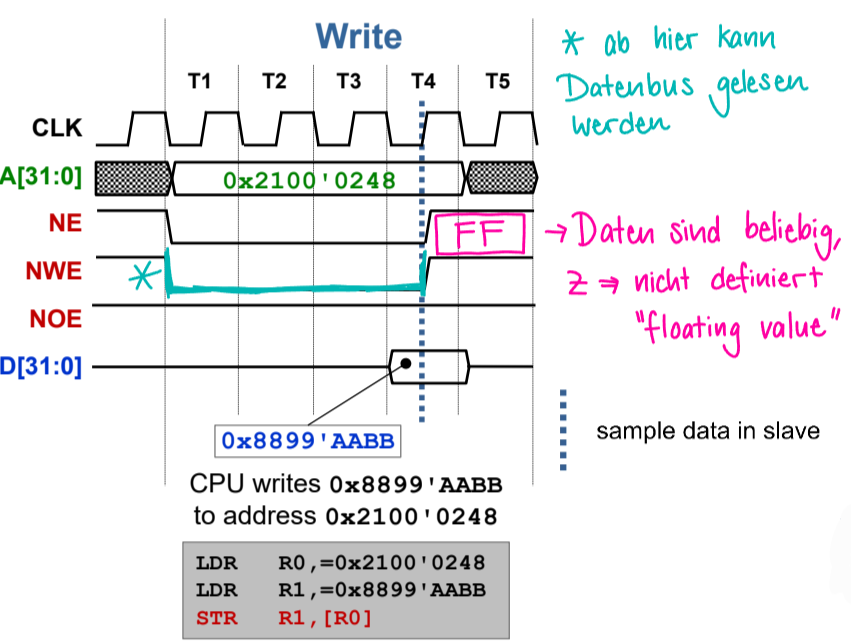
\includegraphics[width=\linewidth]{timing_diagram1.png}

    \begin{minipage}{0.4\linewidth}
        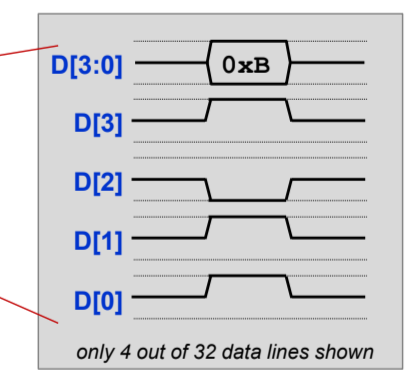
\includegraphics[width=\linewidth]{timing2.png}
    \end{minipage}
    \begin{minipage}{0.54\linewidth}
        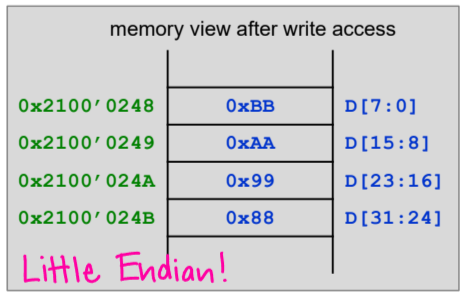
\includegraphics[width=\linewidth]{timing3.png}
    \end{minipage}
    \vspace{1mm}\\
    WICHTIG: nicht genau mit Flanke schreiben, Daten brauchen eine gewisse Zeit um stabil zu werden (keine genaue Definition, muss einfach 'genug' sein)\\
    READ dauert länger als WRITE, da die Daten erst stabil werden müssen bevor sie gelesen werden können
\end{definition}

\begin{theorem}{Bus Timing Diagrams}\\ Notation for Groups of Signals\\
    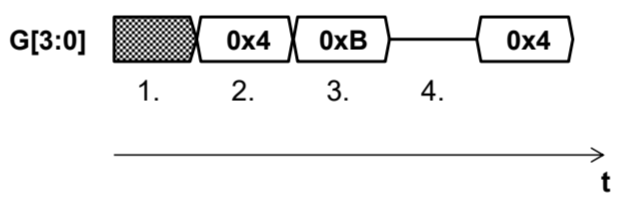
\includegraphics[width=\linewidth]{bus_timing_notation.png}\\
    Group G of 4 signals

1. unknown values

The values on each of the 4 signals are either ' 1 ' or ' 0 ', but unknown.

2. The bus holds the value $0 \times 4$
$$
\text { i.e. } \mathrm{G}[3]=\text { ' } 0 \text { ', G[2] = '1', G[1] = '0', G[0] = '0' }
$$
3. The bus holds the value $0 \times B$
$$
\text { i.e. } \mathrm{G}[3]=\text { ' } 1 \text { ', G[2] = '0', G[1] = '1', G[0] = '1' }
$$
4. Tri-state

All signals $\mathrm{G}[3: 0$ ] are tri-state (i.e. ' $Z$ ' or high-impedance). "No one is driving the bus"
\end{theorem}

\multend



\begin{formula}{Timing Diagram}  
    \begin{itemize}
        \item \texttt{write} \textcolor{darkblue}{D[:]} to \textcolor{darkgreen}{A[:]} $\rightarrow$ \textcolor{darkred}{NE, NWE} = 0
        \item \texttt{read} \textcolor{darkblue}{D[:]} from \textcolor{darkgreen}{A[:]} $\rightarrow$ \textcolor{darkred}{NE, NOE} = 0
    \end{itemize}
    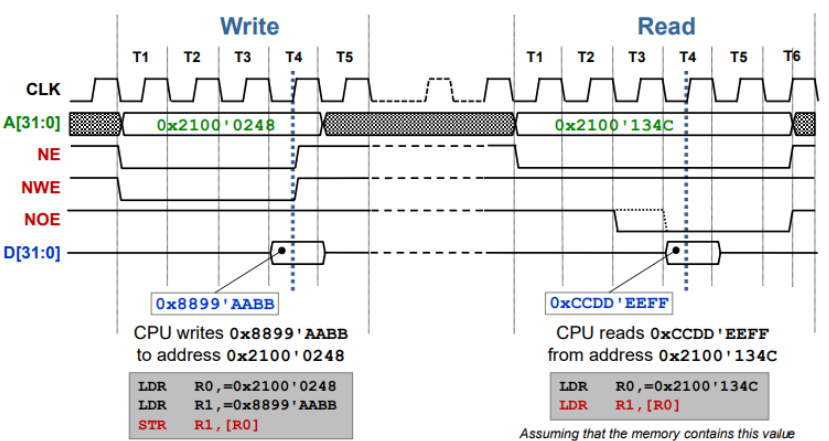
\includegraphics[width=\linewidth]{timing_diagram.png}
\end{formula}




\begin{theorem}{Bus Access Size}
    is determined by the NBL (0-3) (No Byte Line) signals
    \begin{itemize}
        \item NBL = 1 $\rightarrow$ Byte used for Read/Write
        \item NBL = 00
        \item NBL[0:3] = 0011 $\rightarrow$ Read Halfword
        \item NBL[0:3] = 1111 $\rightarrow$ Read Word
    \end{itemize}
    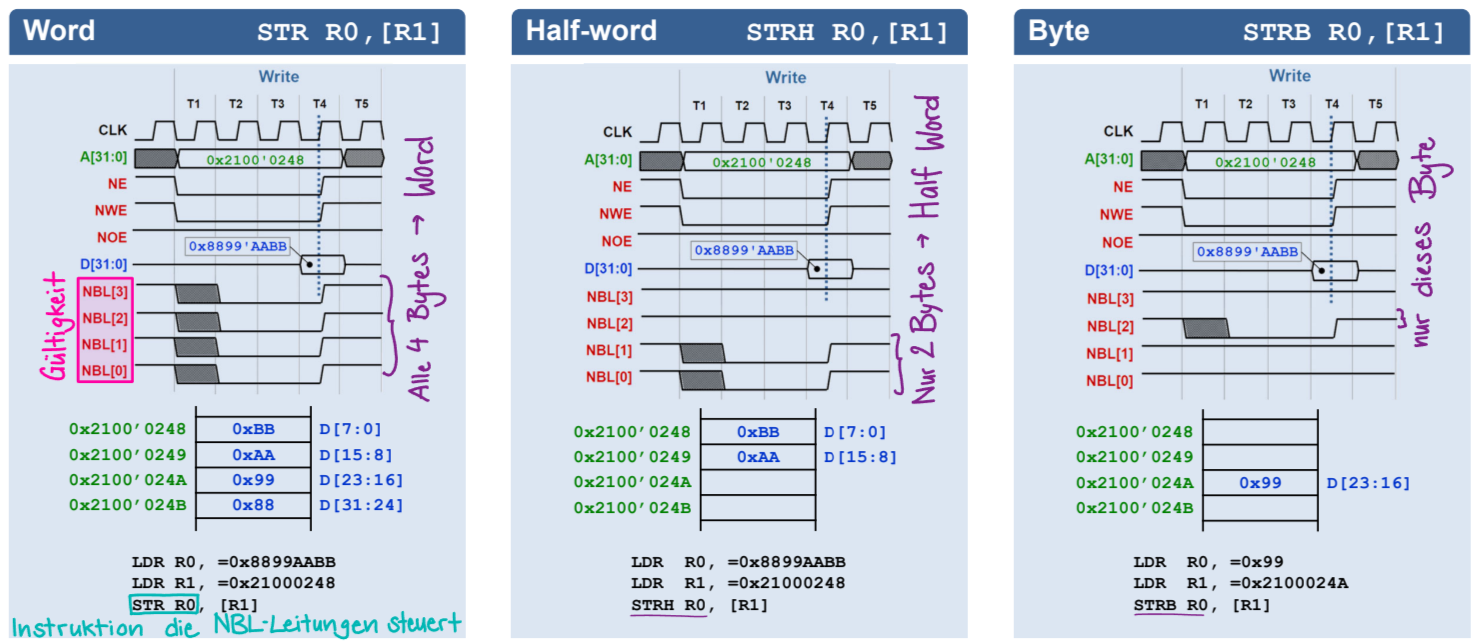
\includegraphics[width=\linewidth]{bus_access_size.png}\\
    Gültigkeit: damit zeigt die CPU an, welche der 4 Bytes übertragen werden sollen (gültig = 0 (unten))\\
    \begin{itemize}
        \item Exact Position of falling edge on NBL varies with chip version
        \item Value on unused data lines are unknown, figues show assumptions
    \end{itemize}
\end{theorem}


\subsection{Control and Status Registers}

\begin{definition}{Hardware Slave (Peripheral)}\\
    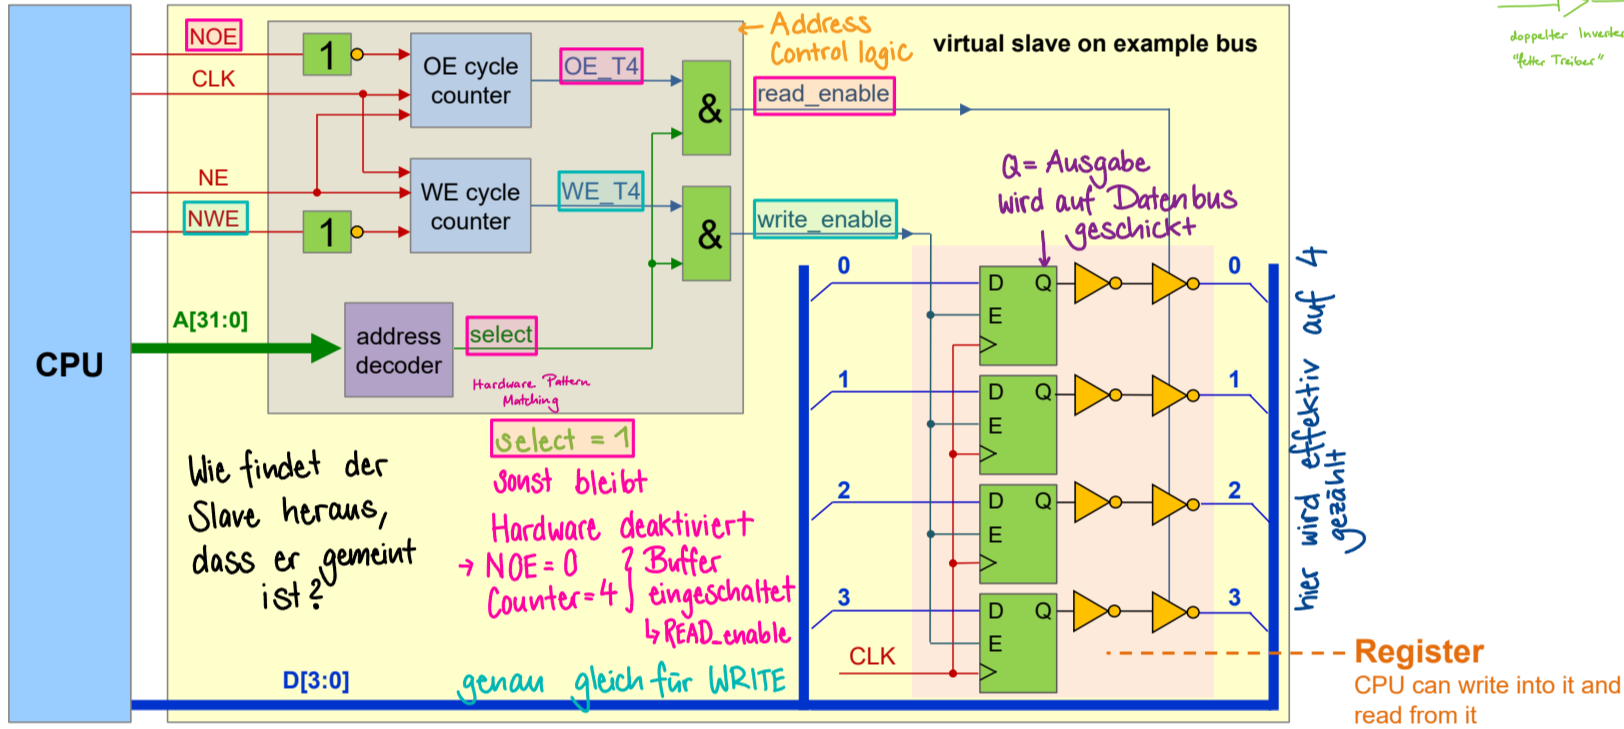
\includegraphics[width=\linewidth]{hardware_slave.png}
\end{definition}

\mult{2}

\begin{concept}{Control Bits}
    \begin{itemize}
        \item Allow CPU to configure Slaves
        \item CPU writes to register bit to configure Slave
        \item Slave uses output of register bit to configure itself
        \item Example: SPI Slave Select (SS) bit
        \item Usually read/write access to control bits
    \end{itemize}
\end{concept}

\begin{concept}{Status Bits}
    \begin{itemize}
        \item Allow CPU to monitor Slaves
        \item CPU reads register bit to monitor Slave
        \item Slave uses input of register bit to monitor itself (Slave writes to register bit)
        \item Example: SPI Busy bit
        \item Usually read-only access to status bits
    \end{itemize}
\end{concept}

\multend

\begin{example}
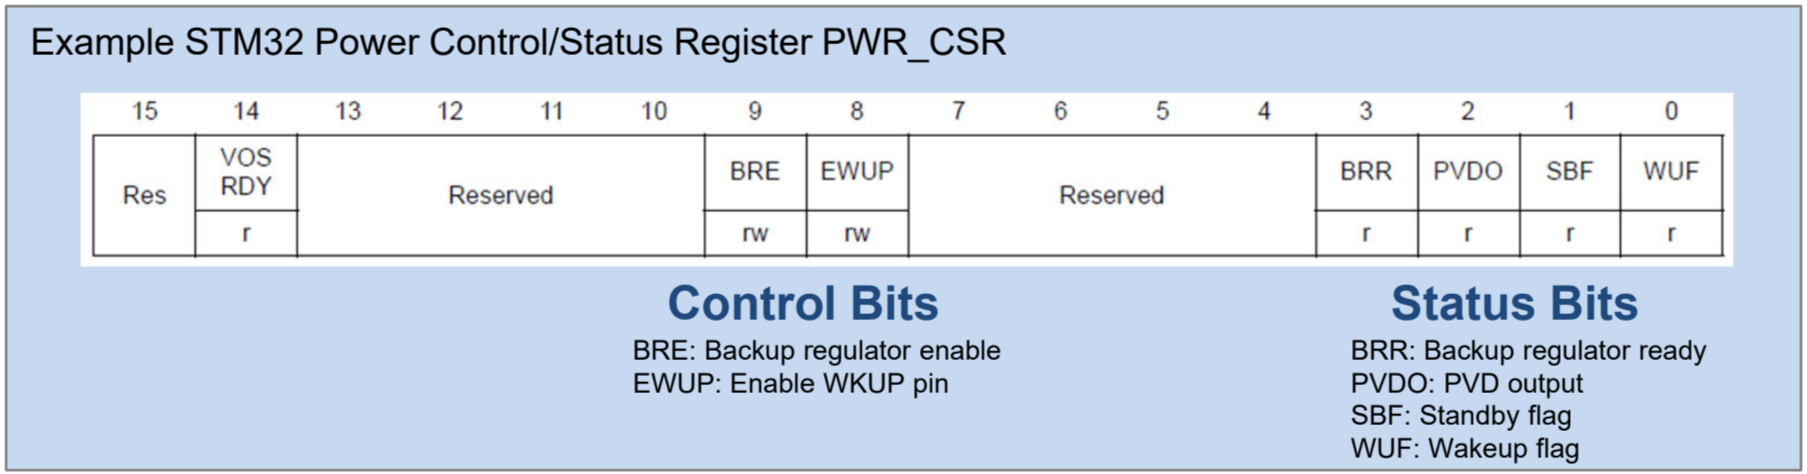
\includegraphics[width=\linewidth]{example_control_status_regs.png}\\
Control/Status register on example bus:

\begin{minipage}{0.5\linewidth}
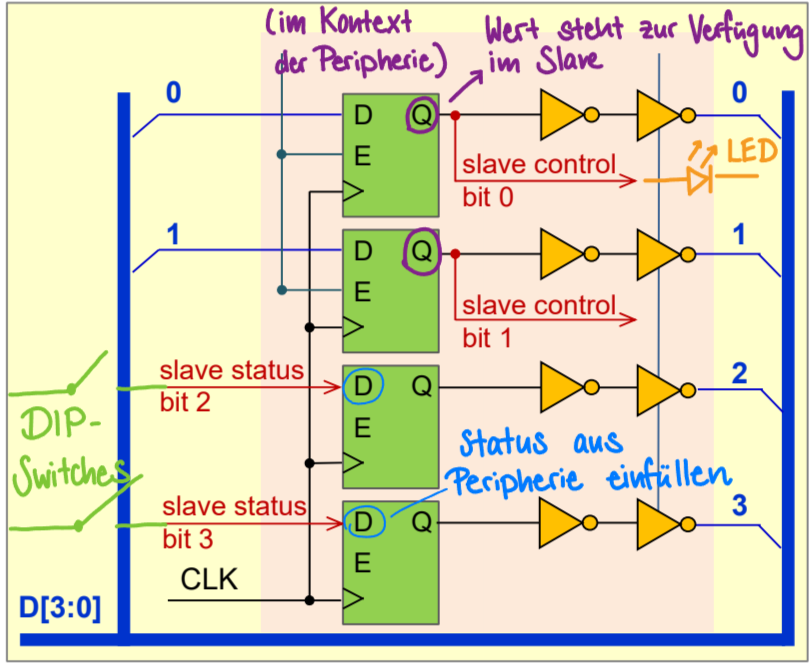
\includegraphics[width=\linewidth]{example_control_status_regs2.png}
\end{minipage}
\begin{minipage}{0.4\linewidth}
control bits: 0 and 1\\
status bits: 2 and 3\\
The same register may contain both control and status bits!
\end{minipage}
\end{example}

\begin{theorem}{Control and Status Registers on CT Board}\\
    Chip-internal and external registers (details on memory map in STM32 Reference Manual)

    \begin{minipage}{0.4\linewidth}
    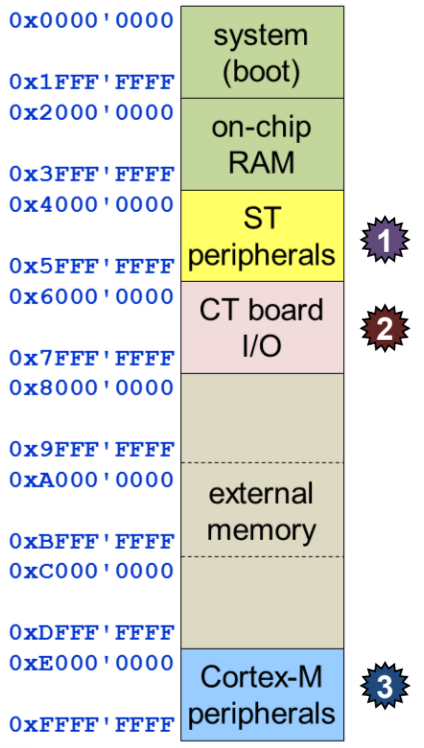
\includegraphics[width=\linewidth]{control_status_regs_ctboard1.png}
    \end{minipage}
    \begin{minipage}{0.54\linewidth}
    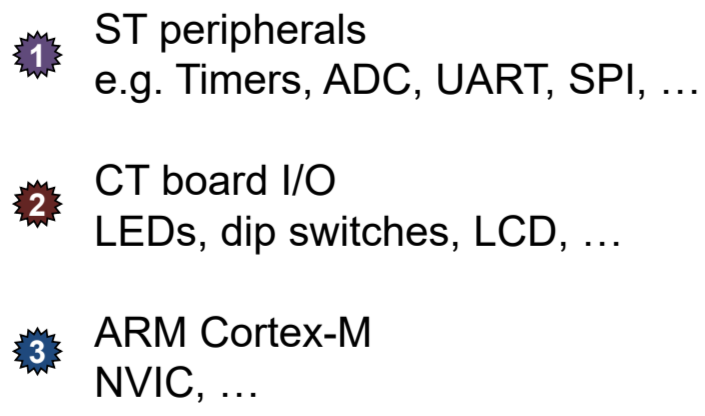
\includegraphics[width=\linewidth]{control_status_regs_ctboard2.png}
    \end{minipage}

    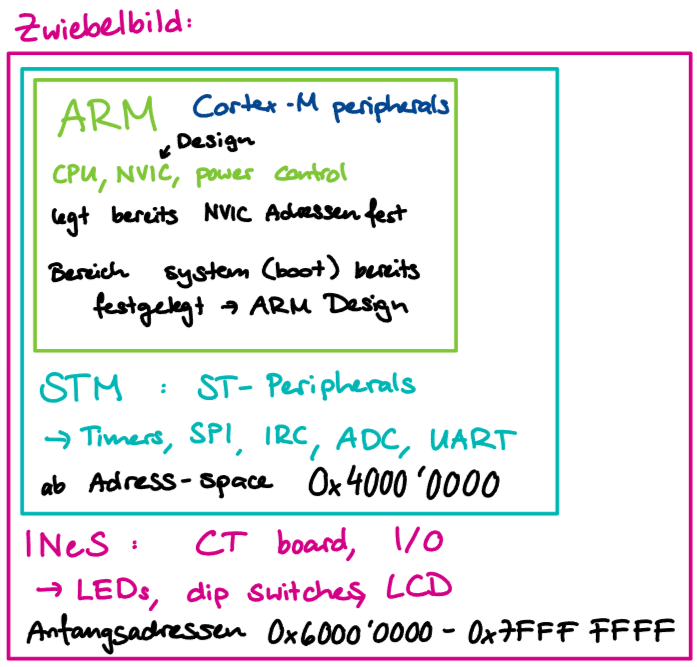
\includegraphics[width=0.6\linewidth]{control_status_regs_ctboard3.png}
\end{theorem}


\subsection{Address Decoding}

\begin{definition}{Address Decoding}\\
    Interpretation of address line values. See whether bus access targets a particular address or address range.
    \begin{itemize}
        \item CPU uses address lines to select a peripheral
        \item Each peripheral has a unique address range
        \item Address decoding logic generates a chip select signal for each peripheral
    \end{itemize}

    \textbf{Full Address Decoding}
    \begin{itemize}
        \item All address lines are decoded
        \item A control register can be accessed at exactly one location
        \item 1:1 mapping: A unique address maps to a single hardware register
        \item example: LEDs and DIP switches on CT board
    \end{itemize}

    \textbf{Partial Address Decoding}
    \begin{itemize}
        \item Only a subset of address lines are decoded
        \item A control register can be accessed at multiple locations
        \item 1:n mapping: Multiple addresses map to the same hardware register
        \item Motivation: Simpler and possible Aliasing (Map a hardware register to several addresses)
    \end{itemize}
    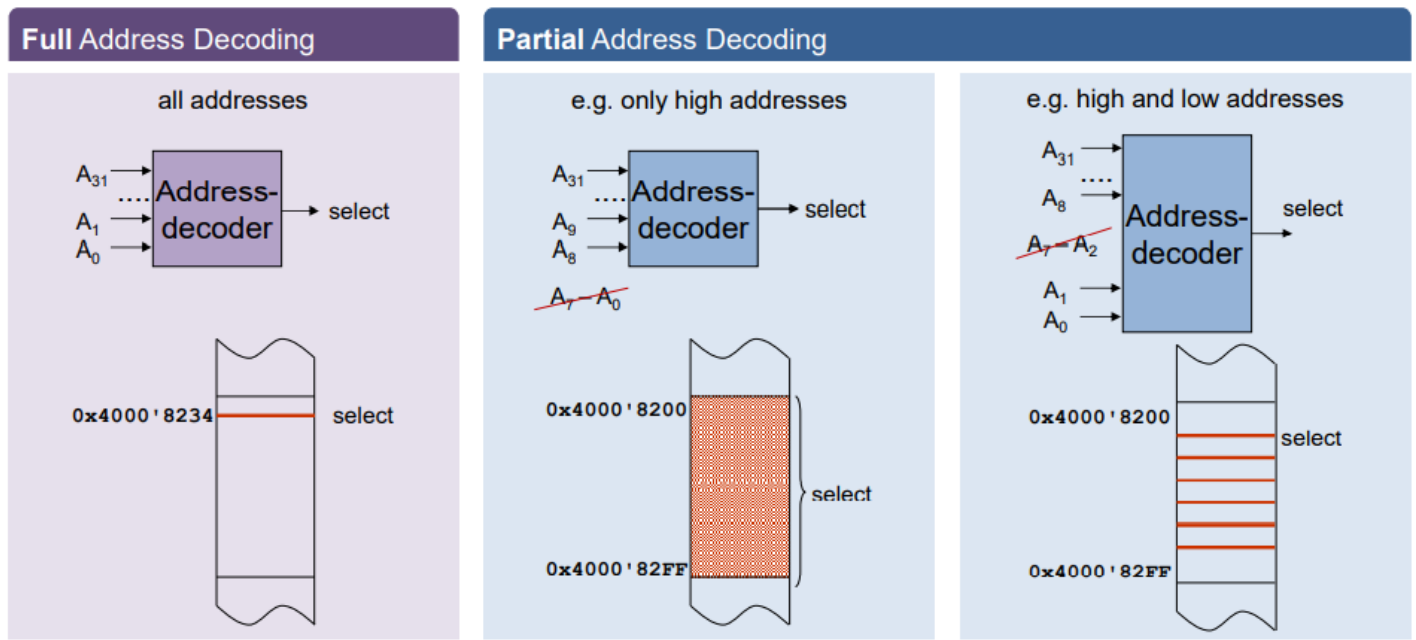
\includegraphics[width=\linewidth]{address_decoding.png}
\end{definition}

\begin{examplecode}{Simple Address Decoder}\\
Basic address decoder with 3 address lines that selects when address is 0x5:
\begin{lstlisting}[language=C, style=basesmol]
// In hardware description language (e.g., Verilog):
assign select = (A[2] & !A[1] & A[0]); // Decodes address 0x5 (101 binary)
\end{lstlisting}
\end{examplecode}

\begin{example2}{Address Decoding Exercise}\\
Given a system bus with 6 address lines A[5:0], determine the address ranges if only bits A[5:4] are decoded.
\tcblower
This means the lower 4 bits (A[3:0]) are not decoded, resulting in a partial address decoding.

Each decoded address represents a range of $2^4 = 16$ addresses.

If A[5:4] = 01, the corresponding address range is:
- Start: 0x10 (binary: 010000)
- End: 0x1F (binary: 011111)

All addresses in this range (0x10 through 0x1F) will select the same device.
\end{example2}

\columnbreak

\begin{theorem}{Address Range Calculation}\\
For partial address decoding, if only higher-order address bits \(A[n:m]\) are decoded (where \(n > m\)), then:
\begin{itemize}
    \item Each decoded address represents a range of \(2^m\) addresses
    \item The size of this address range is \(2^m\) bytes
    \item The start address has all lower bits set to 0
    \item The end address has all lower bits set to 1
\end{itemize}
For example, if only \(A[31:8]\) are decoded, each decoded address represents a 256-byte range (\(2^8 = 256\)).
\end{theorem}

\begin{remark}
    How does a Slave know that it is being addressed?\\
    $\Rightarrow$ Address decoding logic in the Slave (each on its own)
\end{remark}



\begin{example}
    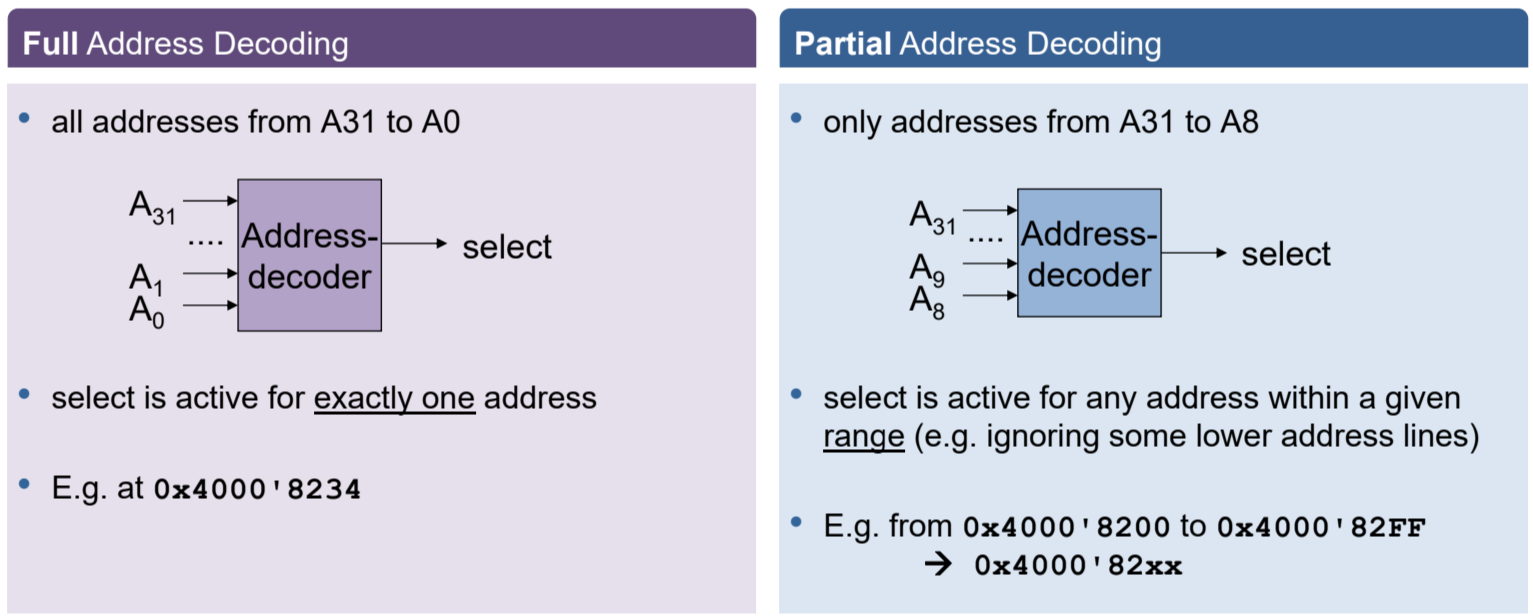
\includegraphics[width=\linewidth]{example_address_decoding.png}\\
    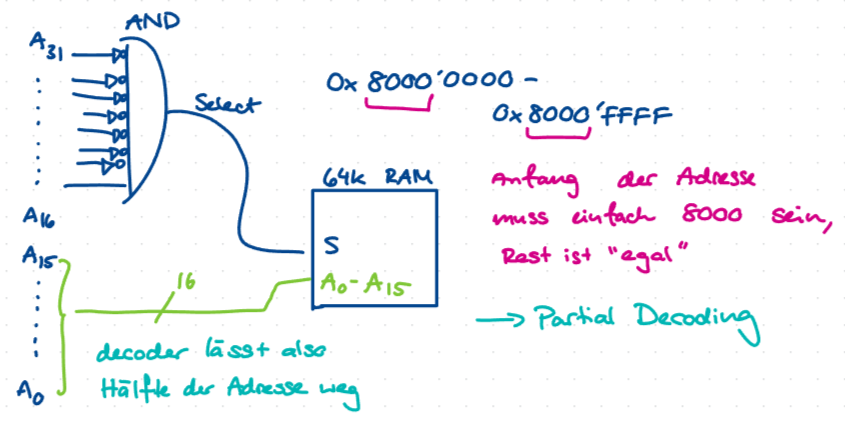
\includegraphics[width=\linewidth]{example_address_decoding2.png}
\end{example}



\columnbreak

\subsection{Wait States for Slow Peripherals}

\begin{definition}{Wait States}\\
Wait states are extra clock cycles inserted to allow slow peripherals to respond.
\begin{itemize}
    \item Without wait states, the slowest slave would determine bus cycle time
    \item Wait states can be:
    \begin{itemize}
        \item Programmed at a bus interface unit depending on the address
        \item Requested by slaves through a "ready" signal (for long or variable access times)
    \end{itemize}
\end{itemize}
\end{definition}

\begin{definition}{Slow Slaves}\\
    Problem: Individual Slave Access times
    \begin{itemize}
        \item If slowest slave defines bus cycle time $\rightarrow$ reduced bus performance
        \item How can we get an individual bus cycle time for each slave?
    \end{itemize}   
\end{definition}

\begin{concept}{Solutions for slow slaves} two possibilities:
    \begin{itemize}
        \item \textbf{Individual Wait States} can be programmed at a bus interface unit \\
        Insert wait states to slow down the CPU to match the speed of the slowest peripheral (depending on the address of an access/bus cycle)\\
        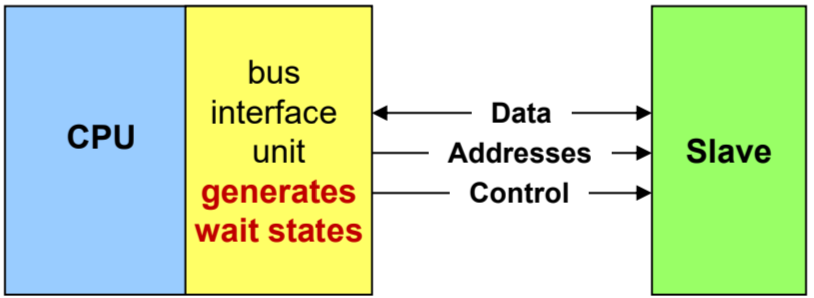
\includegraphics[width=\linewidth]{individual_wait_states.png}
        \item \textbf{Bus Mastering} Slave tells bus interface unit when it is ready \\
        Allow a peripheral to take control of the bus and perform its own accesses (e.g. DMA)\\
        Well suited for slaves with long or variable access times\\
        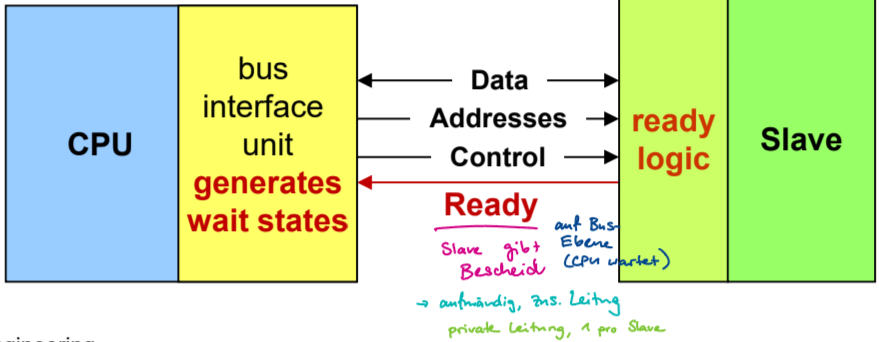
\includegraphics[width=\linewidth]{solution_for_slow_slaves.png}
    \end{itemize}
\end{concept}

\begin{KR}{Individual Wait States}\\
    Wait states are inserted to slow down the CPU to match the speed of the slowest peripheral (depending on the address of an access)

    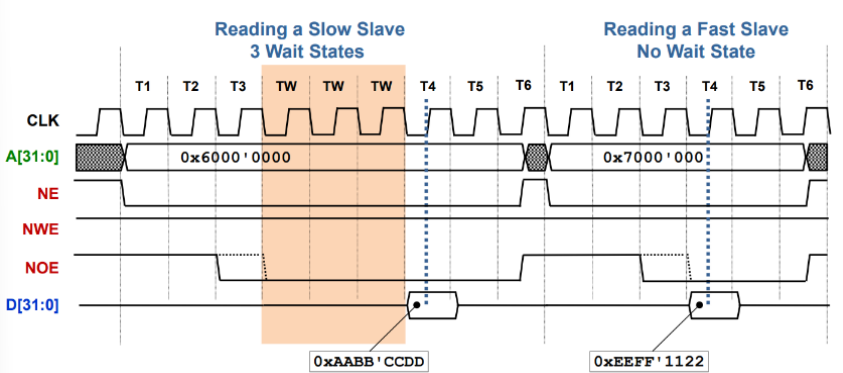
\includegraphics[width=\linewidth]{slow_slaves.png}    
\end{KR}

\subsubsection{Bus Hierarchies}

\begin{example2}{STM32 Microcontroller}\\
    with CPU, on-chip memory, and peripherals interconnected through the system bus(es)
    \begin{itemize}
        \item On-chip system bus: 32 data lines, 32 address lines and control signals
        \item Off-chip external bus: 16 data lines, 24 address lines and control signals
    \end{itemize}
    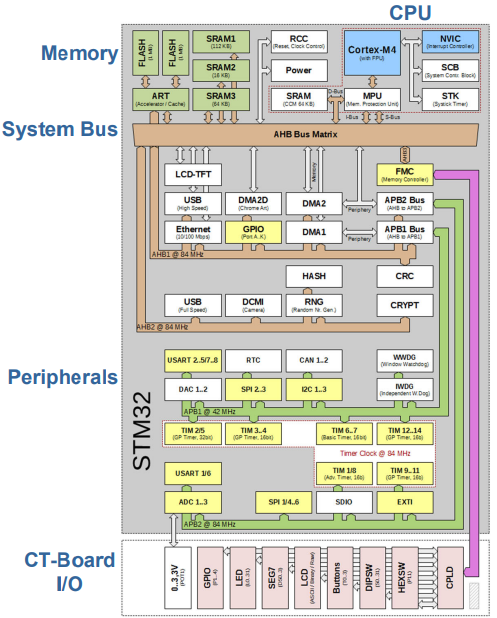
\includegraphics[width=0.9\linewidth]{stm32_example.png}

    A distributed system with parallel (simultaneous) processing of data in many peripherals. All under the supervision of the CPU.
\end{example2}

\begin{remark}
    Note: ARM calls their system buses AHB (ARM High-performance Bus) and APB (ARM
    Peripheral Bus). On complex chips, it is state-of-the-art to partition the system bus into
    multiple interconnected buses.
\end{remark}

\begin{example2}{CT Board with STM32 Microcontroller and Buses}\\
    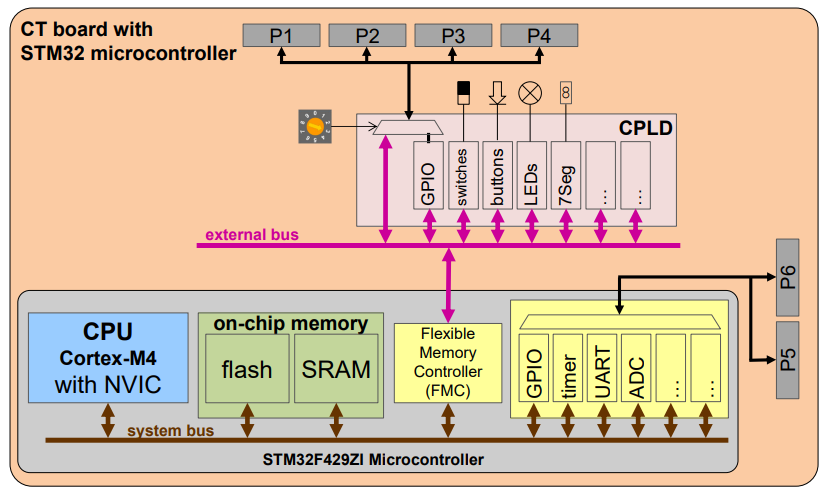
\includegraphics[width=\linewidth]{ctboard_with_stm32.png}\\
    Real-world Systems are partitioned into multiple buses.
\end{example2}

\columnbreak

\subsection{Programming Memory-Mapped Peripherals}

\subsubsection{Accessing Control Registers in C}

\mult{2}

\begin{definition}{Accessing Control Registers in C}\\
    \textbf{Hardware View}
    \begin{itemize}
        \item Signals
        \item Timing
        \item Address decoding
        \item Wait states
        \item Control and status registers
    \end{itemize}
    \textbf{Software View}
    \begin{itemize}
        \item Accessing control and status registers in C
    \end{itemize}
\end{definition}

\begin{concept}{Accessing Control Registers in C}\\
Key considerations:
\begin{itemize}
    \item Compiler optimization may remove statements that appear to have no effect
    \item Register accesses have side effects that the compiler doesn't understand
    \item Use \texttt{volatile} qualifier to prevent compiler optimization
\end{itemize}
\end{concept}

\multend

\begin{concept}{Problem}\\
    Compiler may remove statements that have no effect from the compiler's point of view\\
    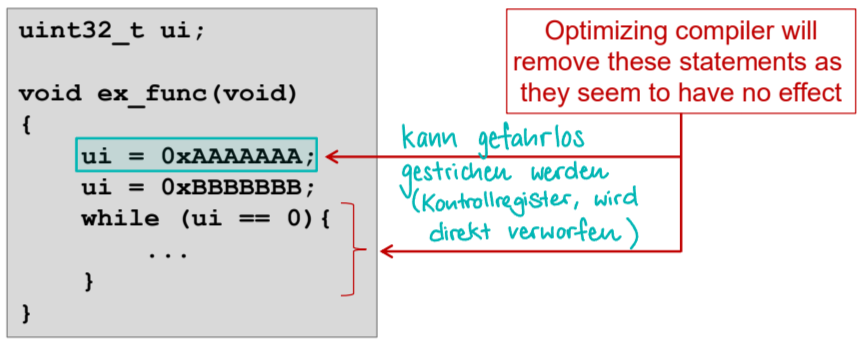
\includegraphics[width=0.7\linewidth]{compiler_problems.png}
    \begin{itemize}
        \item Accesses to control registers (read/write) are memory accesses
        \item If writing has a side effect on the hardware and/or if reading may result in a different value than was set before in the code,
        the program will not behave as intended/expected
    \end{itemize}
\end{concept}

\begin{theorem}{Solution}
    \begin{itemize}
        \item Use the \texttt{volatile} keyword/qualifier in C to prevent the compiler from removing statements that have no effect from the compiler's point of view\\
        $\rightarrow$ prohibit compiler optimizations on the variable\\
        \item The compiler will not optimize away accesses to a variable declared as volatile
        \item The compiler will not reorder accesses to a variable declared as volatile
    \end{itemize}
    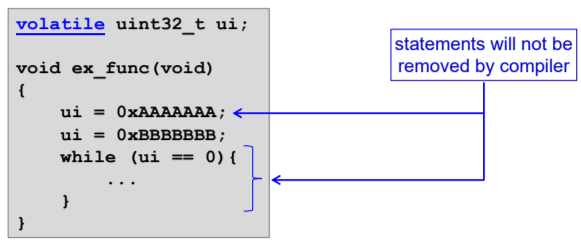
\includegraphics[width=0.7\linewidth]{volatile_keyword.png}
    \begin{itemize}
        \item Tell compiler that the variable may change at any time, outside the control of the compiler (e.g. by hardware or interrupt handler)
        \item The compiler cannot make any assumptions about the value of the variable\\
        needs to execute all read/write accesses as programmed\\
        prevents compiler optimizations
    \end{itemize}
\end{theorem}

\begin{code}{Using volatile for register access}
\begin{lstlisting}[language=C, style=basesmol]
// Without volatile, compiler might remove these statements
uint32_t ui;
void ex_func(void) {
    ui = 0xAAAAAAA;  // Appears to have no effect
    ui = 0xBBBBBBB;  // Appears to have no effect
    while (ui == 0) {
        // ...
    }
}

// With volatile, all accesses are preserved
volatile uint32_t ui;
void ex_func(void) {
    ui = 0xAAAAAAA;  // Will be executed
    ui = 0xBBBBBBB;  // Will be executed
    while (ui == 0) {
        // ...
    }
}
\end{lstlisting}
\end{code}

\begin{KR}{Accessing Registers Through Pointers}
\paragraph{Step 1: Create pointer to register}
Define a pointer to a volatile memory-mapped register.
\paragraph{Step 2: Assign address}
Cast the register's physical address to a pointer type.
\paragraph{Step 3: Access register}
Use pointer dereference to read or write.

\begin{lstlisting}[language=C, style=basesmol]
// Create a pointer to volatile uint32_t
volatile uint32_t *p_reg;

// Set LEDs
p_reg = (volatile uint32_t *)(0x60000100);
*p_reg = 0xAA55AA55;  // Write pattern to LEDs

// Wait for DIP switches to be non-zero
p_reg = (volatile uint32_t *)(0x60000200);
while (*p_reg == 0) {
    // Wait until any switch is pressed
}
\end{lstlisting}
\end{KR}

\begin{corollary}{Access through Pointers} e.g. writing to and reading from CT Board I/O

    \begin{minipage}{0.6\linewidth}
    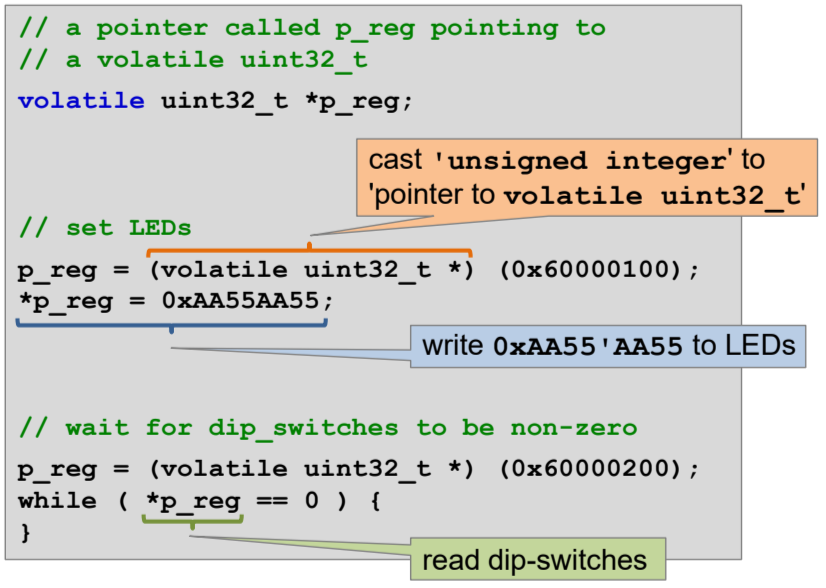
\includegraphics[width=0.9\linewidth]{access_through_pointers1.png}
    \end{minipage}
    \begin{minipage}{0.2\linewidth}
    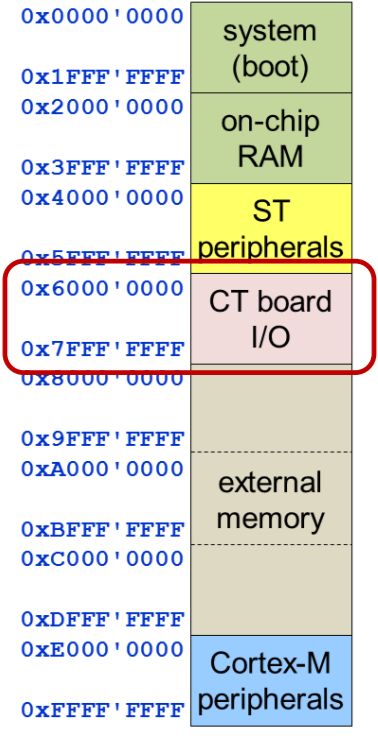
\includegraphics[width=\linewidth]{access_through_pointers2.png}
    \end{minipage}
\end{corollary}

\begin{KR}{Using Preprocessor Macros for Register Access}
\paragraph{Step 1: Define register macros}
Create macros that encapsulate register addresses with proper casting and dereferencing.
\paragraph{Step 2: Use macros for access}
Access registers through the defined macros.

\begin{lstlisting}[language=C, style=basesmol]
// Define register macros
#define LED31_0_REG     (*((volatile uint32_t *)(0x60000100)))
#define BUTTON_REG      (*((volatile uint32_t *)(0x60000210)))

// Write to LED register
LED31_0_REG = 0xBBCCDDEE;

// Read button register
uint32_t aux_var = BUTTON_REG;
\end{lstlisting}
\end{KR}

\begin{examplecode}{Using Preprocessor Macros} $\rightarrow$ \#define
\begin{lstlisting}[language=C, style=basesmol]
#define LED31_0_REG (*((volatile uint32_t *) 0x60000100))

#define BUTTON_REG (*((volatile uint32_t *) 0x60000210))

//Write LED register to 0xBBCC'DDEE
LED31_0_REG = 0xBBCCDDEE;
//Read Button register to aux_var
aux_var = BUTTON_REG;
\end{lstlisting}
    \vspace{2mm}
    \texttt{(\textcolor{darkturquoise}{*}(\textcolor{pink}{(volatile\ uint32\_t *)} 0x60000100))}\\
    $\rightarrow$ \textcolor{darkturquoise}{dereference} the pointer to the register address\\
    $\rightarrow$ \textcolor{pink}{cast} the address to a pointer to a 32-bit register
\end{examplecode}

\raggedcolumns
\columnbreak

\section{Microcontroller Basics Exercises}

\subsection{Bus Access Analysis}

\begin{KR}{Analyzing Bus Cycle Diagrams}
\paragraph{Read access analysis}
\begin{itemize}
    \item Examine clock (CLK), address lines (A), data lines (D), and control signals (NWE, NOE, NE)
    \item Identify whether it's a read (NOE active) or write (NWE active) operation
    \item Note the address value from address lines
    \item For read operations, note the data value returned on data lines
\end{itemize}

\paragraph{Write access analysis}
\begin{itemize}
    \item Identify write operations (NWE active)
    \item Note the address value from address lines
    \item Note the data value being written from data lines
\end{itemize}

\paragraph{Memory mapping}
\begin{itemize}
    \item Remember that processors like ARM use little-endian ordering
    \item Lowest memory address holds the least significant byte (LSB)
    \item Highest memory address in the word holds the most significant byte (MSB)
    \item Map the bytes according to this ordering in memory
\end{itemize}
\end{KR}

\begin{example2}{Bus Cycle Analysis Example}\\
Given the following bus cycle diagram, determine the operation type, address, and data value:

\begin{center}
\begin{tabular}{l}
Access 1: T1 T2 T3 T4 T5 T6 with A[31:0] = 0x6100ABC8, NOE active, D[31:0] = 0x11223344 \\
Access 2: T1 T2 T3 T4 T5 with A[31:0] = 0x6100ABC8, NWE active, D[31:0] = 0x55667788
\end{tabular}
\end{center}

\tcblower
\paragraph{Solution:}
Access 1: This is a read operation because NOE is active.
\begin{itemize}
    \item Address: 0x6100ABC8
    \item Data read: 0x11223344
\end{itemize}

Access 2: This is a write operation because NWE is active.
\begin{itemize}
    \item Address: 0x6100ABC8
    \item Data written: 0x55667788
\end{itemize}

Memory contents (little-endian):
\begin{center}
\begin{tabular}{|c|c|}
\hline
\textbf{Address} & \textbf{Content before Access 2} \\
\hline
0x6100ABC8 & 0x44 (LSB) \\
0x6100ABC9 & 0x33 \\
0x6100ABCA & 0x22 \\
0x6100ABCB & 0x11 (MSB) \\
\hline
\end{tabular}
\quad
\begin{tabular}{|c|c|}
\hline
\textbf{Address} & \textbf{Content after Access 2} \\
\hline
0x6100ABC8 & 0x88 (LSB) \\
0x6100ABC9 & 0x77 \\
0x6100ABCA & 0x66 \\
0x6100ABCB & 0x55 (MSB) \\
\hline
\end{tabular}
\end{center}
\end{example2}

\subsection{Address Decoding}

\begin{KR}{Analyzing Address Decoding Logic}
\paragraph{Identifying addressable range}
\begin{itemize}
    \item Determine the total address space from the number of address lines: $2^n$ bytes
    \item For partial address decoding, identify which address lines are actually decoded
    \item Find which address bits are fixed (compared in the logic) and which are "don't care"
\end{itemize}

\paragraph{Calculating address ranges}
\begin{itemize}
    \item For fully decoded address: Only one specific address activates the select signal
    \item For partially decoded address:
    \begin{itemize}
        \item Identify how many address bits are not decoded ("don't care" bits)
        \item Calculate the number of different addresses that map to the same location: $2^m$ where $m$ is the number of "don't care" bits
        \item Use the fixed bits to determine the base address pattern
        \item Substitute all possible values for the "don't care" bits to find all addresses
    \end{itemize}
\end{itemize}

\paragraph{Creating decoding logic}
\begin{itemize}
    \item For exact address decoding: AND all address bits (or their complements) according to the required pattern
    \item For partial decoding: Only include the relevant address bits in the logic
\end{itemize}
\end{KR}

\begin{example2}{Address Decoding Example}\\
Given a 6-bit address bus A[5:0], determine the addresses that will select a device with the following address decoding logic:
\begin{center}
select = A[5] \& A[4] \& !A[3] \& !A[2]
\end{center}

\tcblower
\paragraph{Solution:}
The decoding logic fixes 4 address bits: A[5:2] = 1100

The bits A[1:0] are "don't care" bits (not included in the logic), giving 4 possible addresses:
\begin{itemize}
    \item A[5:0] = 110000 = 0x30
    \item A[5:0] = 110001 = 0x31
    \item A[5:0] = 110010 = 0x32
    \item A[5:0] = 110011 = 0x33
\end{itemize}

Therefore, the device can be addressed at any of these four addresses: 0x30, 0x31, 0x32, or 0x33.
\end{example2}

\columnbreak

\subsection{Memory-Mapped I/O Access in C}

\begin{KR}{Memory-Mapped Register Access in C}
\paragraph{Define register addresses}
\begin{itemize}
    \item Use \texttt{\#define} for each register address
    \item Create pointer types for each data width (8-bit, 16-bit, 32-bit)
    \item Use \texttt{volatile} qualifier to prevent optimization
\end{itemize}

\paragraph{Reading from registers}
\begin{itemize}
    \item Cast the register address to a volatile pointer of appropriate width
    \item Dereference the pointer to read the value
    \item Use bit masks and shifts to extract specific bits if needed
\end{itemize}

\paragraph{Writing to registers}
\begin{itemize}
    \item Cast the register address to a volatile pointer of appropriate width
    \item Assign a value to the dereferenced pointer to write
    \item For bit manipulation operations:
    \begin{itemize}
        \item Use bitwise OR (|) to set specific bits without affecting others
        \item Use bitwise AND (\&) with inverted mask to clear specific bits
        \item Use bitwise XOR ($\land$) to toggle specific bits
    \end{itemize}
\end{itemize}

\paragraph{Waiting for status bits}
\begin{itemize}
    \item Create a polling loop that checks the status bit
    \item Use appropriate bit masks to isolate the status bit
    \item Use volatile to ensure the register is read on each iteration
\end{itemize}
\end{KR}

\begin{example2}{Memory-Mapped Register Access Example}\\
Write C code to:
\begin{enumerate}
    \item Read an 8-bit control register at address 0x61000007
    \item Set all bits of a 16-bit control register at address 0x61000008 to '1'
    \item Wait until bit 15 in a 32-bit register at address 0x6100000C is set
    \item Set bit 16 in a 32-bit register at address 0x61000010 without changing other bits
\end{enumerate}

\tcblower
\paragraph{Solution:}
\begin{lstlisting}[language=C, style=basesmol]
#include <stdint.h>

// Define register addresses with appropriate types
#define MY_BYTE_REG     (*((volatile uint8_t *)(0x61000007)))
#define MY_HALFWORD_REG (*((volatile uint16_t *)(0x61000008)))
#define MY_WORD_REG     (*((volatile uint32_t *)(0x6100000C)))
#define MY_WORD_REG2    (*((volatile uint32_t *)(0x61000010)))

void register_operations(void) {
    // Read 8-bit control register
    uint8_t my_var = MY_BYTE_REG;
    
    // Set all bits of 16-bit register to '1'
    MY_HALFWORD_REG = 0xFFFF;
    
    // Wait until bit 15 is set in 32-bit register
    while (!(MY_WORD_REG & 0x00008000)) {
        // Empty loop body
    }
    
    // Set bit 16 without changing other bits
    MY_WORD_REG2 |= 0x00010000;
}
\end{lstlisting}
\end{example2}

